\chapter[Proposed RL-based FLSO algorithm]{Proposed RL-based FLSO algorithm}

\section{System model}
\quad This thesis considers a large-scale LEO satellite constellation deployed across $P$ orbital planes, represented by the set $\mathcal{P} = \left\{p \mid p = 1, \dots, P\right\}$. The constellation consists of $N$ LEO satellites in total, distributed across these planes, with $N_p$ satellites in plane $p$. We write the overall satellite index set as $\mathcal{S} = \{ s_{p,i} \mid p = 1, \dots, P;\ i = 1, \dots, N_p \}$, and its cardinality as $\lvert\mathcal{S}\rvert = \sum_{p=1}^{P} N_p$. For simplicity in the following equations, we denote a single satellite by its global index $n \in \{1, \dots, N\}$. The LEO satellite $n$ connects to ground GWs via feeder link, where the set of GWs is denoted as $\mathcal{G} = \left\{m \mid m = 1, 2, \dots, M\right\}$. The coordinates of each LEO satellite $n$ in the Earth-centered, Earth-fixed (ECEF) coordinate system at a given time slot $t$, where $t \in \{0, 1, \dots, T\}$, are given by $l_n(t) = (x_n(t), y_n(t), z_n(t))$.

The primary challenge addressed in this thesis is GW load balancing. We define the load of a GW \( m \) at time \( t \), denoted as $\mathcal{L}_m(t)$, as the set of satellites $n \in \mathcal{S}$ currently connected to it. The instantaneous load is $\lvert \mathcal{L}_m(t) \rvert$.

\begin{sidewaysfigure}[p]
\centering
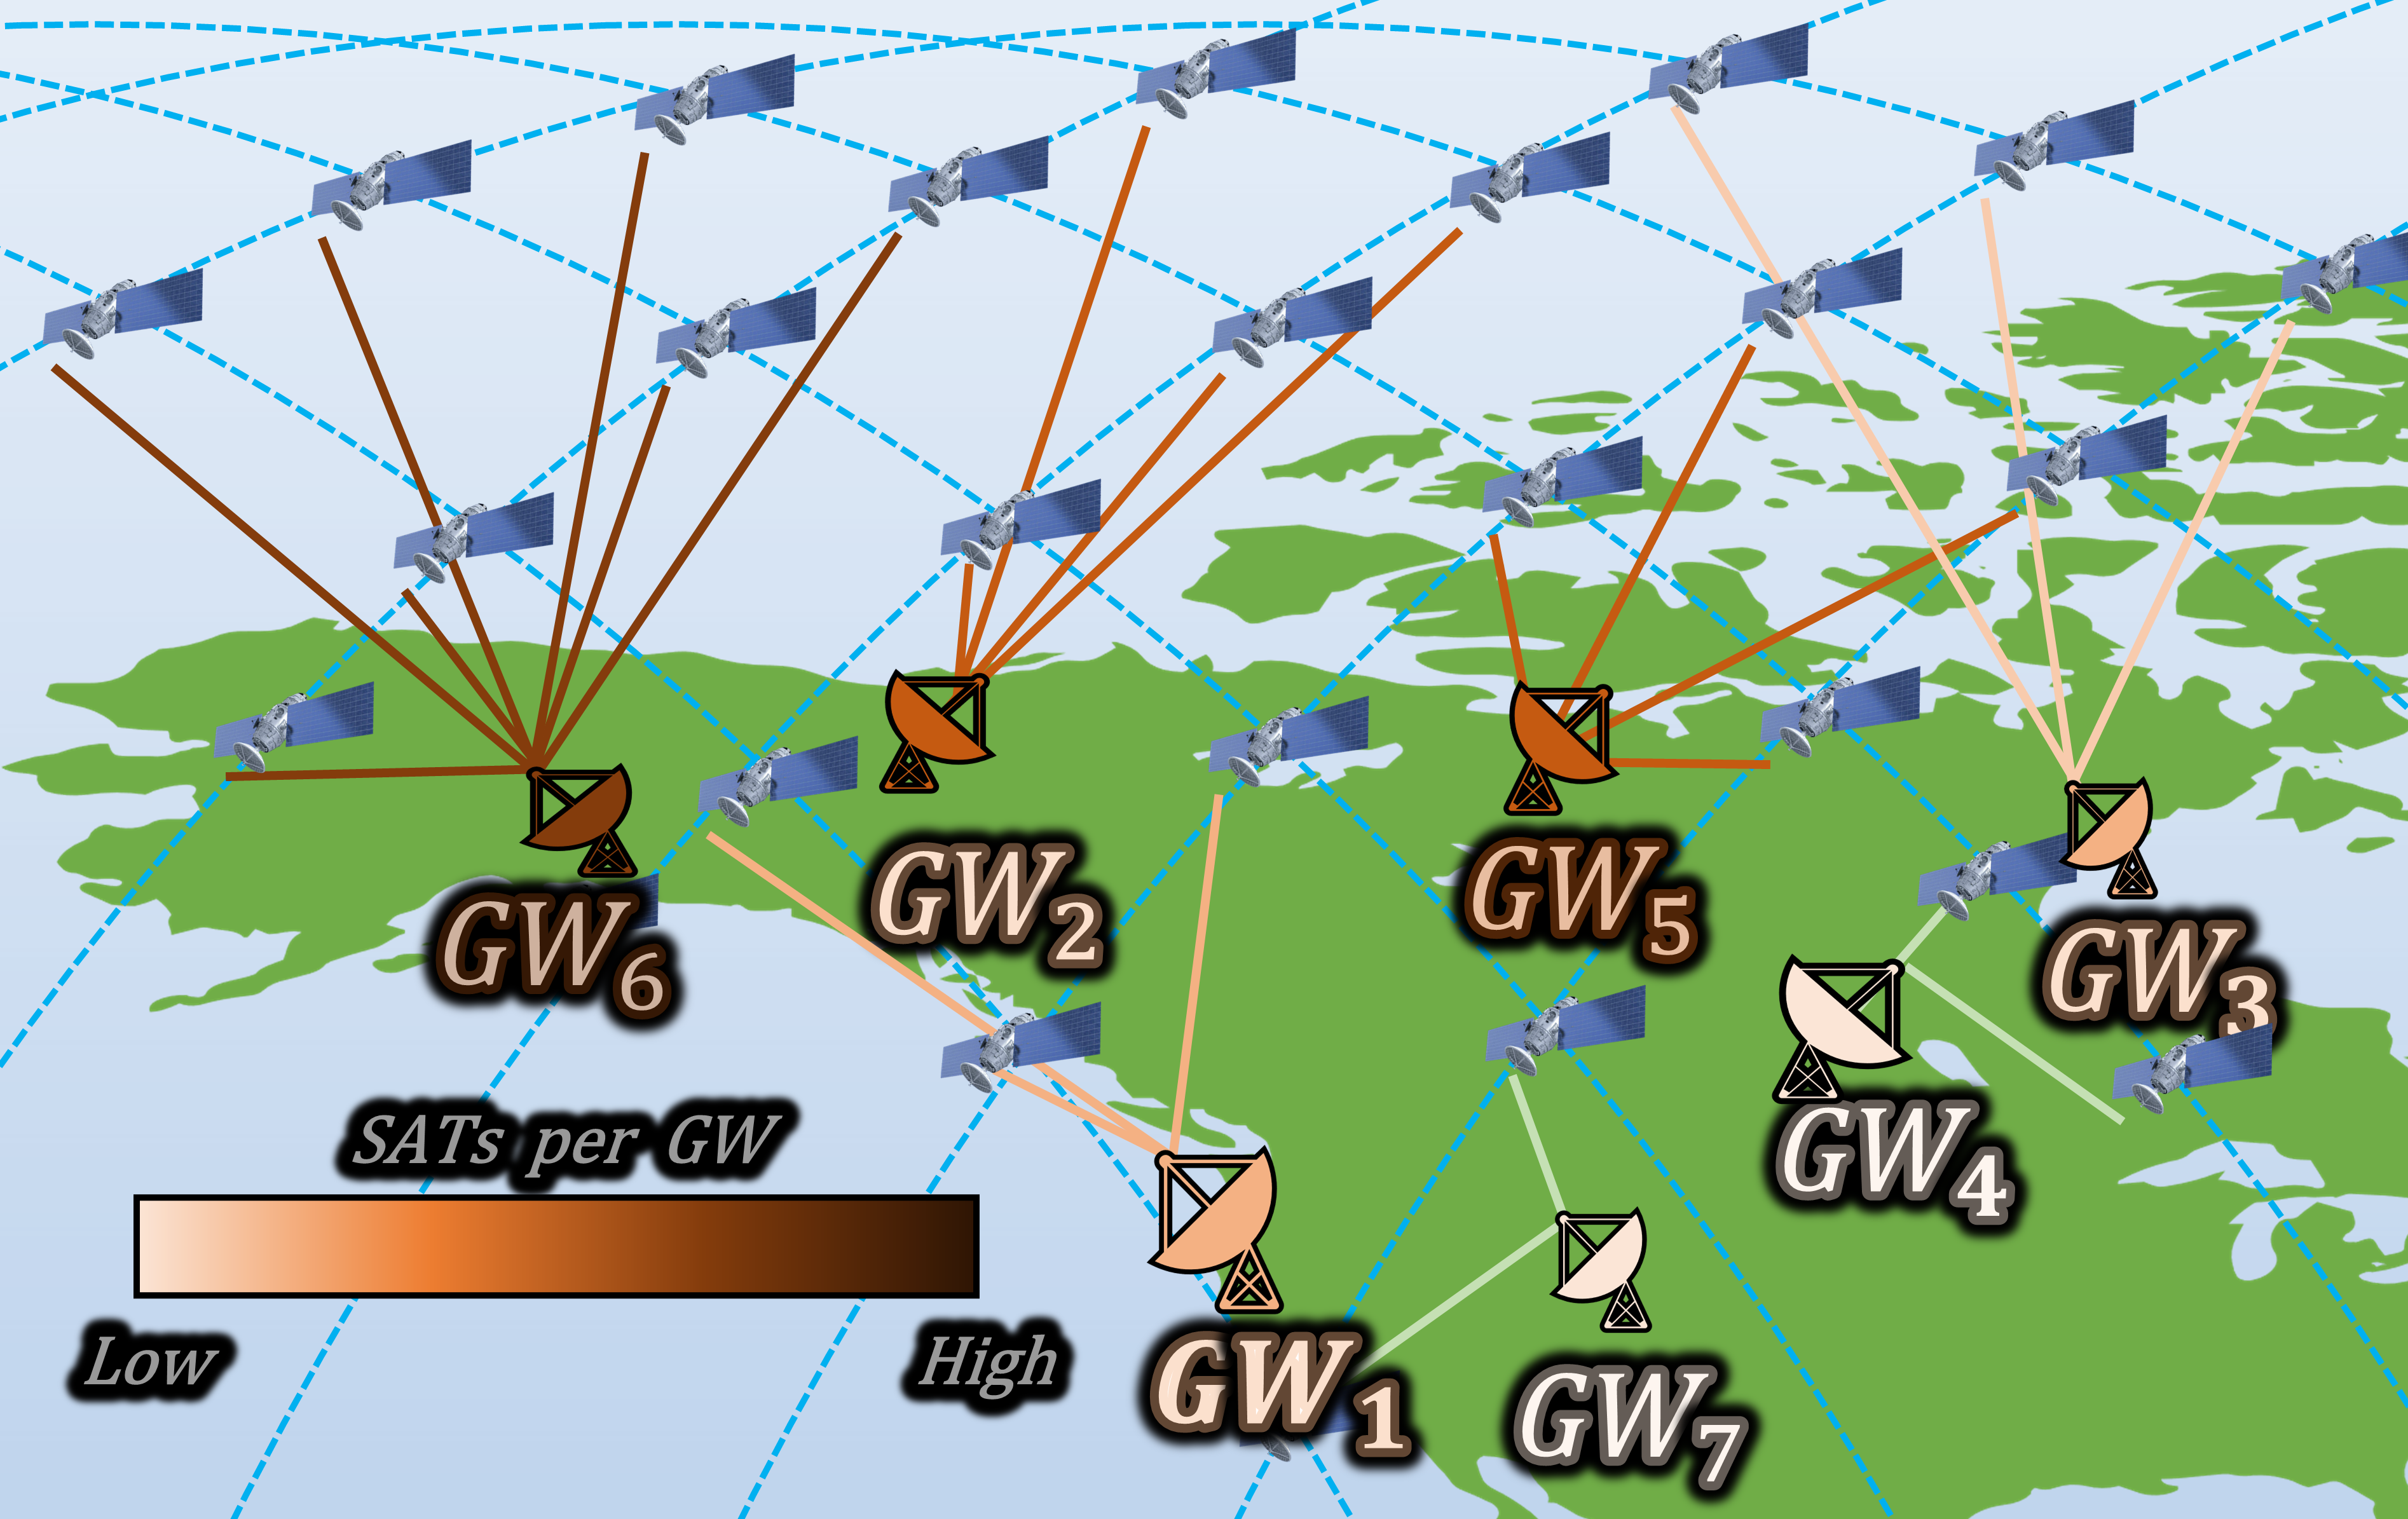
\includegraphics[width=1.0\columnwidth]{figure/fig_system_model.png}
\caption{Network scenario of a LEO satellite performing FLSO while across Starlink GWs in the United States.}
\label{figure_system_model}
\end{sidewaysfigure}

The LEO satellite \( n \) evaluates the RSRP from signals transmitted by the GW \( m \) at periodic interval \( T_m \). The RSRP \( R_{m,n} \) is calculated as follows:
\begin{equation}
R_{m,n} = EIRP_{m} + G_{n} - PL_{m,n} - 10 \log_{10}(q_{RB}),
\label{eq:rsrp}
\end{equation}
where \( EIRP_{m} \) is the effective isotropic radiated power (EIRP) of the GW \( m \), defined as \( EIRP_{m} = P_{m} + G_{m} \), with \( P_{m} \) being the transmit power and \( G_{m} \) the transmit antenna gain of the GW $m$ towards the LEO satellite \( n \). \( G_{n} \) represents the receive antenna gain of the LEO satellite \( n \). The term \( 10 \log_{10}(q_{RB}) \) is used to normalize the RSRP measurement, accounting for a single resource block out of the total resource blocks \( q_{RB} \) allocated to the link. $PL_{m,n}$ is the large-scale path loss between the GW \( m \) and the LEO satellite \( n \), and this expression is adapted from 3GPP documentation \cite{3gppchanel}. The model is calculated as follows:
\begin{align}
&PL_{m,n} = P_{{LOS,{m,n}}} \big( FSPL_{m,n}(d_{m,n}, f_m) + SF_{m,n} \big)\notag\\
&\quad + P_{{NLOS,{m,n}}} \big( FSPL_{m,n}(d_{m,n}, f_m) + SF_{m,n} + CL_{m,n}  \big) + AT_{m,n},
\end{align}
$P_{{LOS,{m,n}}}$ and $P_{{NLOS,{m,n}}}$ denote the probabilities that the LEO satellite \( n \) to GW \( m \) is in a line-of-sight (LoS) and non-line-of-sight (NLoS) condition, respectively. $FSPL_{m,n}(d_{m,n}, f_m)$ denotes the free space path loss (FSPL) as a function of the distance $d_{m,n}$ between the LEO satellite \( n \) and the GW \( m \) and the frequency $f_m$ of the GW \( m \) uplink feeder link frequency. $SF_{m,n}$ represents the shadow fading, which accounts for the signal attenuation caused by obstacles such as buildings, trees, or terrain variations in the propagation path. $CL_{m,n}$ denotes the clutter loss, reflecting additional signal degradation due to environmental clutter. $AT_{m,n}$ captures atmospheric attenuation along the feeder link slant path, including gaseous absorption due to dry air and water vapor, and it can be obtained from standard ITU-R models for the considered band~\cite{ITU-R-P.676-13}. Specifically, the $FSPL_{m,n}$ is calculated as follows:
% 한글 주석: 경로손실 식에 대기 감쇄 AT_{m,n}를 추가하여 LOS/NLOS 모두에 반영합니다. (기체 흡수 등, ITU-R 모델 기반 계산 가능)
\begin{equation}
FSPL_{m,n} = 32.45 + 20\log_{10}(f_m) + 20\log_{10}(d_{m,n}).
\end{equation}

At each measurement instant $t$, the LEO satellite \( n \) samples the RSRP from GW \( m \) and all neighboring GWs within instantaneous visibility region, yielding the raw RSRP $R_{m,n}(t)$. To mitigate the effects of shadow fading and measurement noise, these raw RSRP $R_{m,n}(t)$ samples are processed at the radio resource control (RRC) layer using a layer 3 (L3) infinite impulse response (IIR) filter \cite{3gppl3}. Denoting the filtered RSRP by $\widetilde{R}_{m,n}(t)$, the update equation is calculated as follows:
\begin{equation}
  \widetilde{R}_{m,n}(t) = a{R}_{m,n}(t) + (1 - a)\widetilde{R}_{m,n}(t-1),
  \label{eq:L3filter_new}
\end{equation}
where $a \in (0,1)$ is the L3 forgetting factor, defined as $a = \left(\frac{1}{2}\right)^{K/4}$, and $K$ is the filter coefficient. The initial condition is set as $\widetilde{R}_{m,n}(0) = R_{m,n}(0)$. Finally, the LEO satellite compiles a measurement report containing the L3-filtered RSRP $\widetilde{R}_{m,n}(t)$ of the serving and neighboring GWs and transmits this report back to the serving GW \( m \) over the feeder link.

% To quantify the link quality during the simulation, we calculate the channel capacity $C$ using the Shannon capacity formula, which is calculated as follows:
% \begin{equation}
% C = B_m \log_2(1+{\zeta}),
% \label{eq:capacity}
% \end{equation}
% where the $B_m$ is the uplink bandwidth of GW \( m \) and $\zeta' is the SNR calculated as follows:
% \begin{equation}
% {\zeta} = {EIRP_{m}}+\frac{G_{n}}{T}-k-{PL_{m,n}}-B_m,
% \label{eq:snr}
% \end{equation}
% where, $k$ is the Boltzmann constant, $G_n/T$ is the antenna gain-to-noise temperature ratio, is calculated as follows:
% \begin{equation}
% \frac{G_n}{T} = G_{n} - N_{f} - 10\log_{10}\left(T_0 + (T_a - T_0) 10^{-0.1 N_{f}} \right),
% \end{equation}
% where $N_{f}$ is LEO satellite noise figure, $T_0$ and $T_a$ is ambient and antenna temperature.



\section{Problem formulation}
\quad In this section, we address the optimization problem for the LEO satellite constellation. The objective is to find an optimal FLSO policy $\pi$ that dynamically assigns each satellite $n \in \mathcal{S}$ to a GW $m \in \mathcal{G}$ at each time slot $t$.

The primary goal is to minimize the overall network load imbalance while simultaneously maximizing the collective link quality RSRP and minimizing the instability caused by frequent FLSOs. We define $m_t^{n}$ as the GW selected by satellite $n$ at time $t$. This problem can be formulated as a multi objective optimization problem.

We define the following cost and reward components for each satellite $n$ at time $t$:

\begin{itemize}
    \item \textbf{FLSO Cost:} A cost $C_{FS}$ is incurred if the satellite switches its serving GW, penalizing instability.
    \begin{equation}
    FS_{m,n}(t) = \begin{cases} C_{FS} & \text{if } m_t^{n} \neq m_{t-1}^{n}, \\ 0 & \text{otherwise}. \end{cases}
    \label{eq:flso_cost}
    \end{equation}

    \item \textbf{UFLSO Cost:} A cost $C_{UFS}$ is incurred for an unnecessary FLSO (UFLSO), which occurs if the satellite switches to another GW within a minimum time-of-stay (MTS), denoted $\tau_{min}$. Let $\tau_{stay}(t)$ is the time elapsed since the last FLSO.
    \begin{equation}
    UFS_{m,n}(t) = \begin{cases} C_{UFS} & \text{if } m_t^{n} \neq m_{t-1}^{n} \text{ and } \tau_{stay}(t) < \tau_{min}, \\ 0 & \text{otherwise}. \end{cases}
    \label{eq:uflso_cost}
    \end{equation}
    
    \item \textbf{ToS Reward:} A reward is gained for maintaining a connection with the same GW, proportional to the duration of the connection.
    \begin{equation}
    ToS_{m,n}(t) = \tau_{stay}(t).
    \label{eq:tos_reward}
    \end{equation}

    \item \textbf{Load Imbalance Cost:} A cost $\lvert \mathcal{L}_m(t) \rvert$ is incurred for connecting to a congested GW, proportional to the number of satellites already connected.
    
    \item \textbf{Link Quality Reward:} A reward is gained based on the L3-filtered RSRP from the selected GW.
    \begin{equation}
    R_{m,n}(t) = \widetilde{R}_{m,n}(t).
    \label{eq:rsrp_reward}
    \end{equation}
\end{itemize}

The global optimization problem \textbf{P1} is to find the policy $\pi$ that minimizes the total expected cumulative cost and maximizes rewards for all $N$ satellites over the time horizon $T$.

\begin{align}
& \textbf{P1:}\quad \operatorname*{\min}_{\pi} \mathbb{E} \sum_{t=0}^{T} \sum_{n=1}^{N} \sum_{m=1}^{M} \gamma^t \left[ w_{S} \Big( FS_{m,n}(t) + UFS_{m,n}(t) \Big) \right. \notag \\
& \hspace{10em} \left. - w_{T} ToS_{m,n}(t) + w_{L} \lvert \mathcal{L}_m(t) \rvert - w_{R} R_{m,n}(t) \right],\\
& \quad \text{s.t.} \nonumber \\
& \quad \textbf{C1 :}\quad \theta_{m,n}(t) \geq \theta_{\text {min}}, \quad \forall{n}, \forall{m} \in \mathcal{G}_t^{n}, \forall{t},\\
& \quad \textbf{C2 :}\quad \widetilde R_{m,n}(t) \geq R_{\text {min}}, \quad \forall{n}, \forall{m} \in \mathcal{G}_t^{n}, \forall{t},\\
& \quad \textbf{C3 :}\quad m_t^{n} \in \mathcal{G}_t^{n}, \quad \forall{n}, \forall{t}.
\end{align}

In \textbf{P1}, $w_{S}$, $w_{L}$, and $w_{R}$ are the weighting factors that balance the trade-off between switching stability, load balancing, and link quality. $\gamma \in [0, 1]$ is the discount factor for future costs.

The constraints define the set of available GWs, $\mathcal{G}_t^{n}$, for satellite $n$ at time $t$.
Constraint \textbf{C1} ensures the elevation angle $\theta_{m,n}(t)$ to an available GW $m$ exceeds the minimum threshold $\theta_{\min}$, guaranteeing a reliable LoS.
Constraint \textbf{C2} ensures the filtered RSRP $\widetilde{R}_{m,n}(t)$ from an available GW exceeds the minimum required signal quality $R_{\min}$.
Constraint \textbf{C3} mandates that each satellite $n$ must select a GW $m_t^{n}$ from the set of currently available GWs $\mathcal{G}_t^{n}$ that satisfy C1 and C2.

This problem is characterized by high-dimensional state spaces and complex, time-varying dynamics, making it non-deterministic polynomial-time hard (NP-hard)~\cite{singlemachine}. We therefore model this problem as a Markov decision process (MDP) to find an optimal FLSO policy using RL techniques.

\section{Proposed method}
\quad To address the problem \textbf{P1}, we transform it into a dynamic programming framework to derive an optimal FLSO policy. We model the FLSO optimization problem as an MDP due to its ability to handle sequential decision-making in dynamic environments.


\subsection{MDP modeling}
\quad The LEO satellite's state $s_t$ evolves over time and actions $a_t$ impact the future reward $r_t$ with discount factor $\gamma$~\cite{intro_RL}. This MDP formulation enables the agent to jointly account for geometric visibility, link quality, and GW load. At each step $t$, the state of satellite $n$ is defined as
\begin{align}
    s_t = \big\{ l_n(t),\, m_{t},\, \widetilde{R}_{m,n}(t),\, c_{m}(t) \big\},
\end{align}
where $l_n(t)$ denotes the ECEF position of satellite $n$, $m_{t}$ is the index of the serving GW selected at the current step, $\widetilde{R}_{m,n}(t)$ is the L3-filtered RSRP from that serving GW, and $c_{m}(t) \in [0,1]$ is the normalized backhaul complexity of the serving GW. The complexity term $c_m(t)$ is obtained by mapping the instantaneous or pre-estimated number of attached satellites at GW $m$ to a dimensionless score in $[0,1]$ via min-max normalization across all GWs, so that higher values indicate more congested GWs. This compact representation provides the DRL agent with a load-aware yet scale-invariant signal, allowing it to avoid persistently overloaded GWs while optimizing FLSO decisions.

The action space \( {a_t} \) involves the LEO satellite $n$ selecting the optimal GW $m \in \mathcal{G}$ at each step. In line with constraints \textbf{C1-C3}, the action space is the set of available GWs that meet the minimum elevation and RSRP thresholds:
\begin{align}
{a_t} &= \{ m_{t} | m_{t} \in \mathcal{G}_{t}^{n} \}.
\end{align}

The action \(a_t\) is the selection of the next GW, $m_t$, from the set of available GWs \( \mathcal{G}_{t}^{n} \).

The immediate reward \(r_{t}\) is formulated to directly optimize the objective function defined in \textbf{P1}. It penalizes FLSO costs and high load connections while rewarding high quality RSRP links and connection stability. It is calculated as follows:
\begin{align}
r_t &= w_{R} R_{m,n}(t) - w_{S} \Big( FS_{m,n}(t) + UFS_{m,n}(t) - ToS_{m,n}(t) \Big) - w_{L} c_{m}(t),
\end{align}
where the cost and reward components are defined in Eq. \eqref{eq:flso_cost} through \eqref{eq:rsrp_reward}, and the weights are the corresponding weights from \textbf{P1}.

Discount factor $\gamma$ is a value between 0 and 1, which represents the rate at which future rewards are discounted when considering them at the current step.

\subsection{Proposed dueling DDQN algorithm}
%복잡도 측면에서 얼마나 걸리는지 설명, GeForce RTX 3080 Ti GPU에서 수 밀리초 내에 행동을 출력할 수 있다.
\label{Proposed Dueling DDQN Algorithm}
\quad In this paper, we employ a RL algorithm to enable LEO satellites to operate in an dynamic environment. As depicted in Fig.\ref{Fig:system_model2}, the architecture of the proposed dueling DDQN algorithm, incorporating a \(\epsilon\)-greedy policy, is designed to optimize FLSO in LEO satellite networks. The LEO satellite receives feedback to execute actions that sustain both a prolonged ToS and an elevated RSRP, while minimizing the frequency of FLSO and, critically, GW congestion. We enhance the traditional DQN framework by incorporating DDQN, prioritized experience replay (PER), and dueling DQN to improve stability, learning efficiency, and robustness against noise in LEO satellite communication systems.

The DQN algorithm \cite{mnih2013playing} approximates the Q-function \( Q(s_t, a_t; \theta) \), which maps a state \( s_t \) and action \( a_t \) to an expected cumulative reward, using a deep neural network (DNN) parameterized by \( \theta \). Two DNNs are utilized: an online network for action selection and a target network for value estimation. The Q-function is trained to minimize the following loss function and loss function is calculated as follows:

\begin{equation}
L(\theta) = \mathbb{E} \left[ \left( y^{DDQN}_t - Q(s_t, a_t; \theta) \right)^2 \right],
\label{eq:loss}
\end{equation}
where the \(y^{DDQN}_t\) is the target and calculated as follows:
\begin{equation}
y^{DDQN}_t = r_t + \gamma \max_a Q(s_{t+1}, \arg\max_{a'} Q(s_{t+1}, a'; \theta); \theta^-),
\label{eq:ddqn_target}
\end{equation}
where \( \theta^- \) represents the parameter of the target network. The target network parameter are updated as \( \theta^- \leftarrow \tau \cdot \theta + (1 - \tau) \cdot \theta^- \), ensuring slow and stable updates to mitigate the moving target problem in the dynamic LEO satellite environment \cite{hazan2019revisiting}.

\begin{sidewaysfigure}[p]
      \centering
      % If the image is missing, show a placeholder box instead of failing the build
      \IfFileExists{figure/dueling_dqn_archi.png}{%
          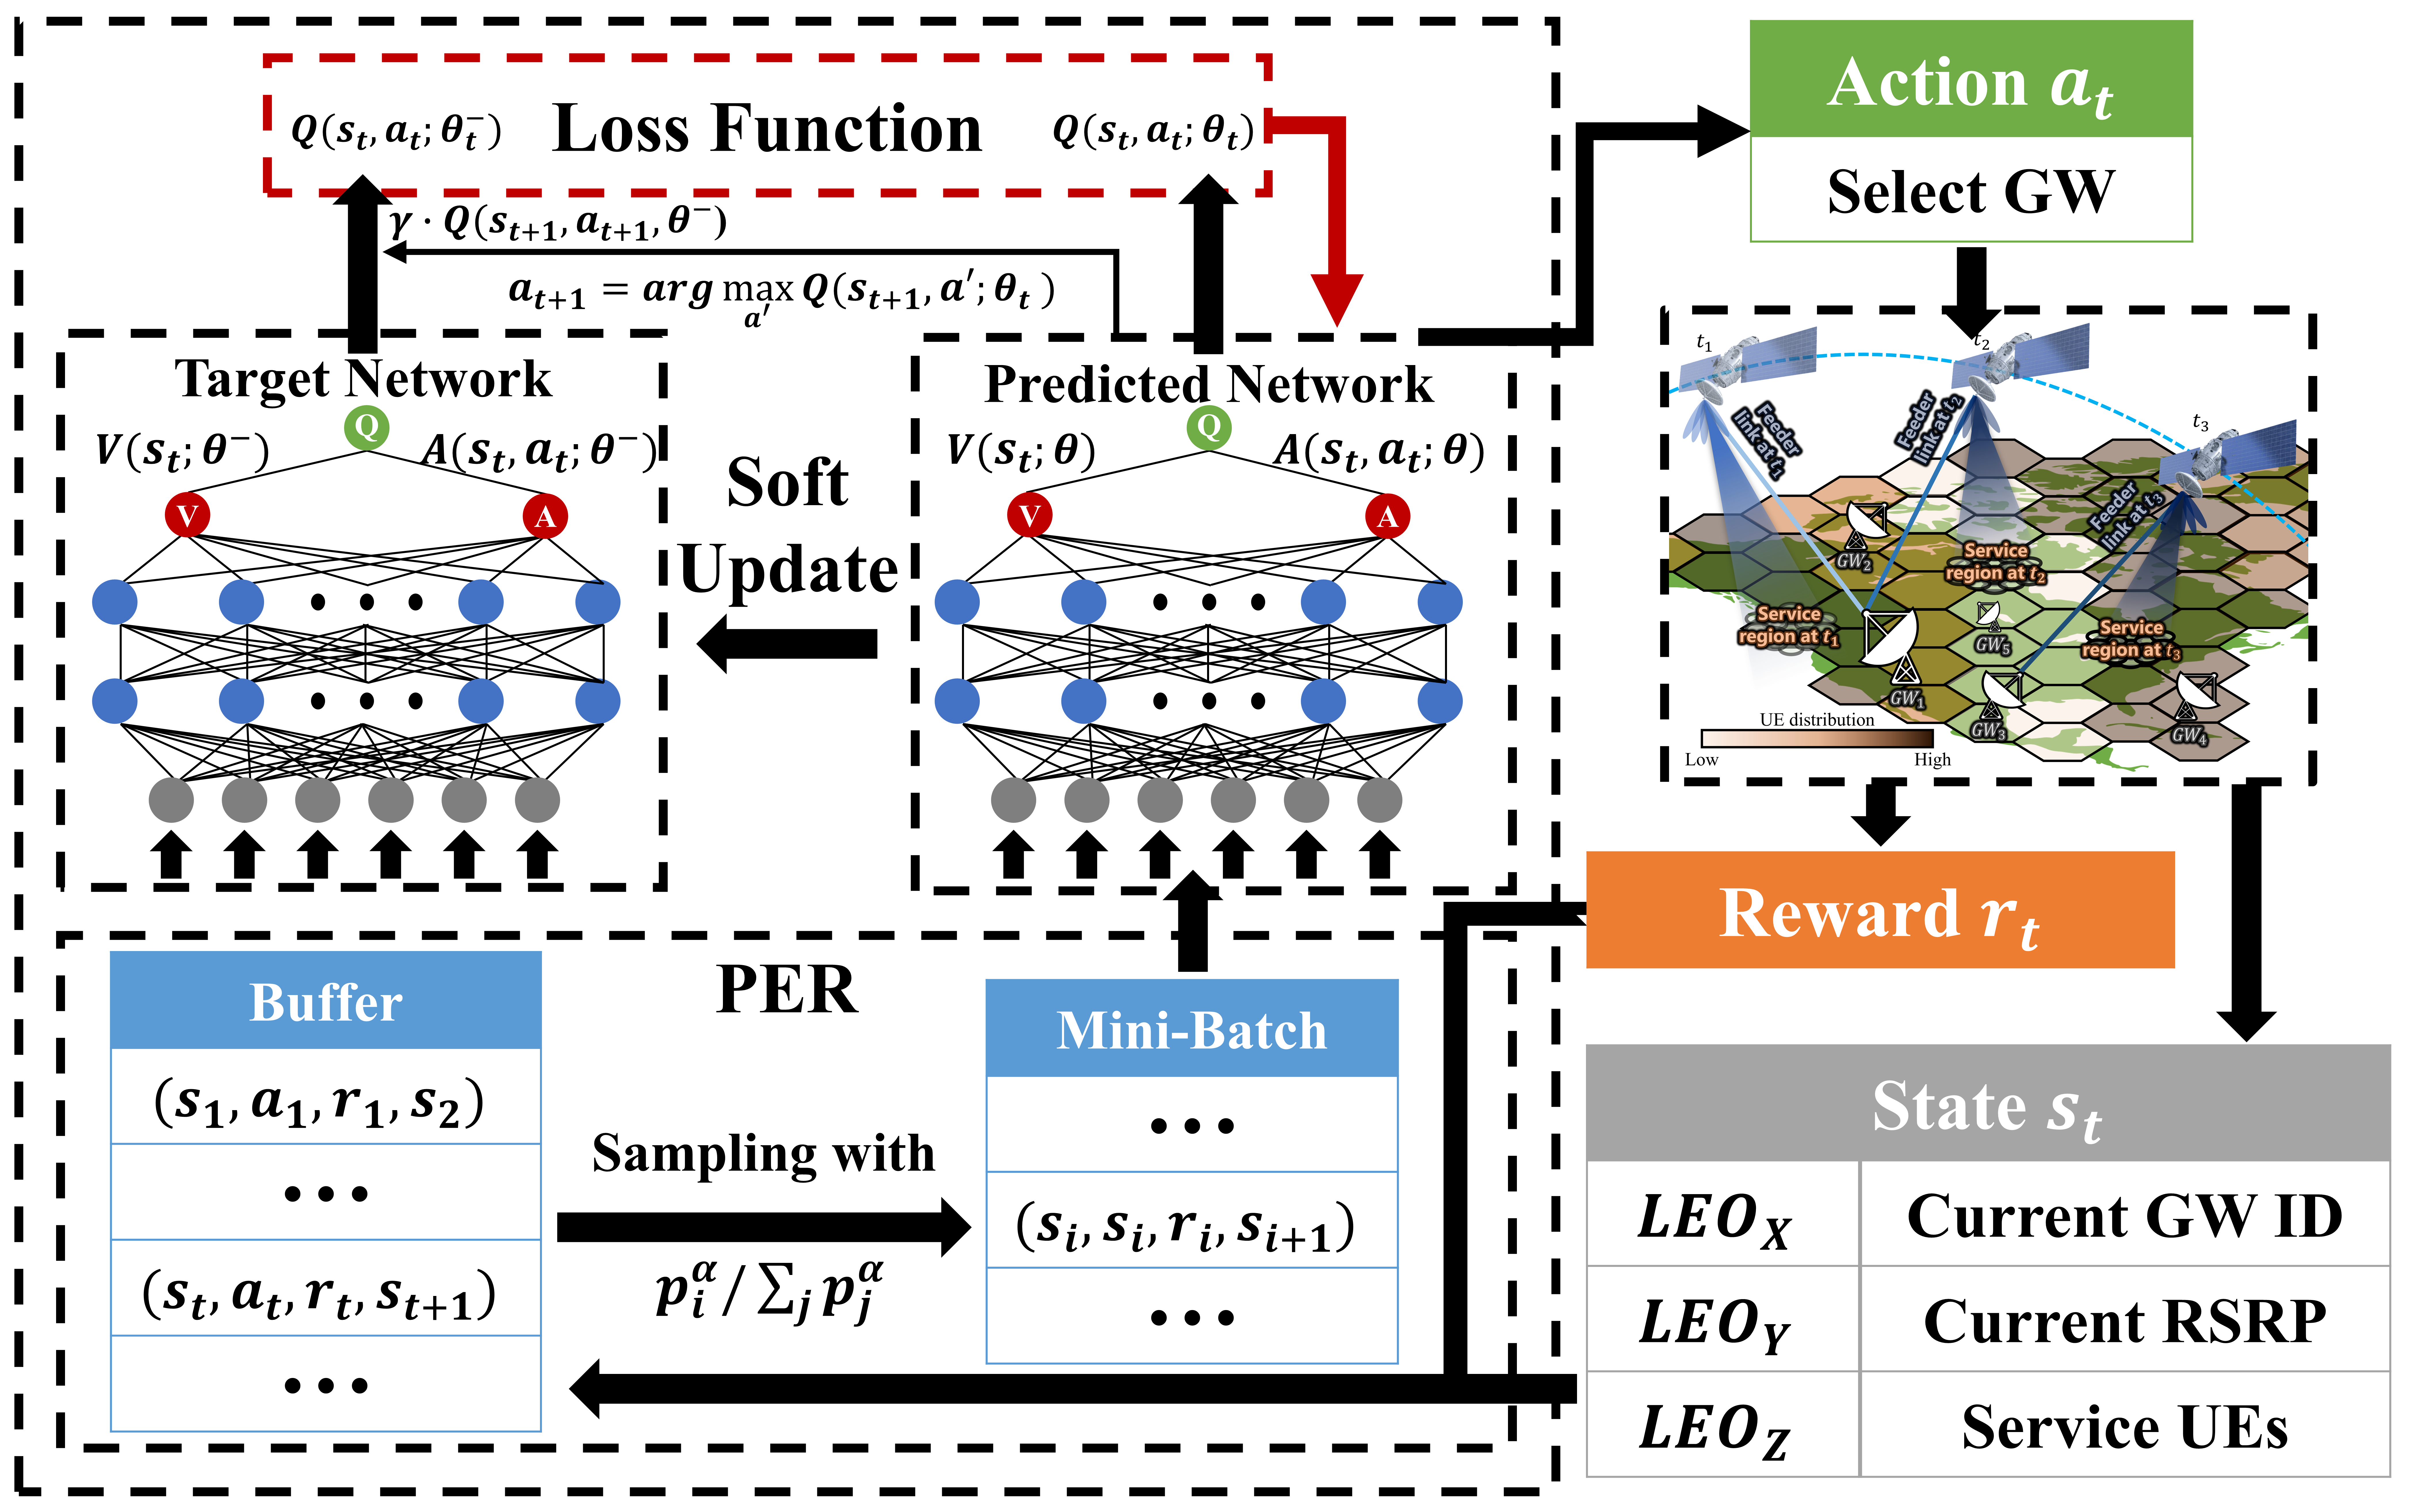
\includegraphics[width=1.0\columnwidth]{figure/dueling_dqn_archi.png}%
      }{%
          \fbox{dueling\_dqn\_archi.png not found}%
      }
      \caption{The architecture of the proposed dueling DDQN for FLSO optimization in LEO satellite networks.}
      \label{Fig:system_model2}
 \end{sidewaysfigure}

To improve robustness against random noise, such as channel shadow fading, we utilize a dueling DQN \cite{wang2016dueling}. The dueling DQN architecture enhances the traditional DQN by splitting the Q-function into two separate streams: the state-value function \( V(s; \theta) \) and the advantage function \( A(s, a; \theta) \). The Q-function is then calculated as follows:
\begin{align}
& Q(s, a; \theta) = V(s; \theta) + \left( A(s, a; \theta) - \frac{1}{|A|} \sum_{a'} A(s, a'; \theta) \right),
\label{eq:dueling_q}
\end{align}
where \( V(s; \theta) \) represents the value of the state \( s \), \( A(s, a; \theta) \) represents the advantage of taking action \( a \) in state \( s \), and \( |A| \) is the number of possible actions. This decomposition allows the network to better distinguish the value of a state from the advantage of each action, improving robustness against noise and enhancing learning efficiency in complex LEO satellite environments.

To further enhance the learning efficiency, we incorporate PER as proposed in \cite{schaul2015prioritized}. PER prioritizes experiences with higher TD errors, where the TD error \(\delta_i\) for transition \(i\) is defined as the difference between the target and current Q-values. The priority is calculated as follows:
\begin{equation}
p_i = |\delta_i| + \epsilon_p,
\label{eq:priority}
\end{equation}
where \( \delta_i = r_i + \gamma Q(s_{i+1}, a_{i+1}; \theta^-) - Q(s_i, a_i; \theta) \) is the TD error, and \( \epsilon_p \) ensures non-zero priorities. PER uses \( \alpha \in [0, 1] \) to control sampling probability \(p_i^\alpha \) and \( \beta \in [0, 1] \) to adjust importance sampling weights \((\mathcal D \cdot P(i))^{-\beta} \), where \( \mathcal D \) is replay buffer limit and \(P(i)\) is the probability of sampling transition \(i\). This approach accelerates learning by focusing on significant transitions, which is beneficial in LEO satellite networks with dynamic and noisy conditions.

By combining dueling DQN with DDQN and PER, our approach effectively addresses overestimation bias, accelerates learning, and mitigates the effects of random noise, leading to improved network performance with effective GW load balancing, elevated RSRP, and reduced FLSO frequency. The detailed process of the training is described in Algorithm \ref{alg:2}.

\begin{algorithm}[p]
\caption{Dueling DDQN-based Algorithm for \textbf{FLSO Load Balancing}}\label{alg:2}
\begin{algorithmic}[1]
    \State \textbf{Initialization:} Random weights $\theta$, replay memory $\mathcal R$ with capacity $\mathcal D$, minibatch size $\mathcal Z$, total episodes $\mathcal E$, prioritization parameter $\alpha$, importance sampling parameter $\beta$, exploration rate $\epsilon$, Polyak averaging parameter $\tau$
    \State \textbf{Input:} State, action, discount factor
    \State \textbf{Output:} Optimal FLSO decision
    \For{$Episode = 1$ to $\mathcal E$}
        \State Initialize the integrated environment
        \For{$t=0$ to $T$}
            \State $a_t = \begin{cases}
            \arg\max_{a'} Q(s_t, a'; \theta) & \text{with } 1 - \epsilon \\
            \text{random action} & \text{with } \epsilon
            \end{cases}$
            \State Execute action $a_t$ (select GW $m_t$), observe reward $r_t$ and next state $s_{t+1}$
            \State Store sample $(s_t, a_t, r_t, s_{t+1})$ into $\mathcal R$
            \If{$|\mathcal R| > \mathcal Z$} \Comment{Start training after buffer fills to batch size}
                \For{$i=1$ to $\mathcal Z$}
                    \State Sample $(s_i, a_i, r_i, s_{i+1})$ from $\mathcal R$ with probability $P(i) = p_i^\alpha / \sum_k p_k^\alpha$
                    \State Calculate DDQN target: $y_i \leftarrow r_i + \gamma Q(s_{i+1}, \arg \max_{a'} Q(s_{i+1}, a'; \theta); \theta^{-})$
                    \State Calculate TD-error: $\delta_i \leftarrow y_i - Q(s_i, a_i; \theta)$
                    \State Update sample priority in $\mathcal R$: $p_i \leftarrow |\delta_i| + \epsilon_p$
                    \State Calculate IS weight: $w_i \leftarrow ((\mathcal D \cdot P(i))^{-\beta}) / \max_j(w_j)$ \Comment{Normalize weight}
                \EndFor
                \State Calculate weighted loss: $L \leftarrow \frac{1}{\mathcal Z} \sum_{i=1}^{\mathcal Z} w_i \cdot \mathcal{L}(\delta_i)$ \Comment{e.g., Huber Loss}
                \State Update online network $\theta$ via gradient descent: $\theta \leftarrow \theta - \eta \nabla_\theta L$
                \State Update target network $\theta^-$ (Polyak averaging): $\theta^- \leftarrow \tau \cdot \theta + (1 - \tau) \cdot \theta^-$
            \EndIf
        \EndFor
    \EndFor
\end{algorithmic}
\end{algorithm}